\part{Introduction}

An embedded system is a combination of hardware and software components put together to achieve a specific task. Often, embedded systems are built into a larger device or system and are used to process data generated within the device and to control the behaviour of the system. Embedded devices are a category of tiny devices with physical, computational, and power constraints that are programmed to perform dedicated tasks.

Like most of the automotive industry, Scania employs embedded devices called \textit{Electronic Control Units} (ECUs) in their trucks to supervise and regulate essential subsystems like the engine, transmission, braking, and electrical systems. Each of these subsystems contain several ECUs to gather system data and transmit it to a central communicator where the sensor data is processed and the system operations are monitored.

Scania currently runs a massive fleet of around 600,000 connected heavy vehicles. The company's truck sales make up 62\% of its global sales and Scania has been adding 60,000 trucks to it's fleet annually \cite{scania-report}. This large fleet of rolling vehicles that are connected though the communicators opens up new possibilities. These connected devices continuously monitor the state of the vehicle and this data can be used to accurately and efficiently schedule vehicle maintainance. For example, if a tire change is predicted to be required in 100 kms then the driver can plan the route smartly to reach the workshop before the vehicle breaks down. This opportunity can be realised by running smart algorithms on the hardware that is currently available.

Machine learning on embedded devices is becoming increasingly popular due to its ability to provide real-time insight and intelligence to devices. This technology can be used to automate tasks, improve efficiency, and make better decisions. But this technology presents a unique set of challenges due to the limited resources available on these devices. Embedded devices are designed to be power efficient, have limited memory and processing power, and require closely tailored algorithms, making it difficult to use pre-existing machine learning models. Furthermore, embedded devices are often expected to produce real-time results, which further complicates the development process. Despite these challenges, machine learning on embedded devices has potential applications in a variety of areas, such as in the fields of robotics and autonomous vehicles.

One such machine learning application that Scania has been developing in their \textsc{LOBSTR} \cite{lobstr} and \textsc{FAMOUS} \cite{famous} projects is \textit{anomaly and fault detection} on the vehicles. Anomalies in this context are patterns in the data that do not conform to the notion of normal behaviour. There are various machine learning techniques available for predicting anomalous behavior in trucks based on the sensor data readings. The running anomaly detection models for fault prediction on the existing ECUs with limited resources has many benefits and challenges.

\subsection*{Benefits to performing Anomaly Detection on ECUs}

\begin{itemize}
	\item Scania is committed to promote a shift towards autonomous and eco-friendly transport systems. The latest addition of Scania's connected trucks and buses will be embedded with upgraded ECUs and communication devices. However, this upgrade will make the stock of older hardware devices to become obsolete and regarded as e-waste, which could be prevented. Exploring the possibility of repurposing existing ECUs to run ML models aligns with Scania's vision of leading the way towards a sustainable future.
	\item Neural networks are a type of machine learning technique that can learn intricate patterns across multiple data signals and time. Neural networks can learn from unstructured data and apply this understanding to unseen data points. Anomaly detection using neural network has the advantage of requiring less manual work in labelling data and can provide paradigms allowing for automation of discovering new and important data points.
	\item Federated learning techniques allow for the ECUs installed in Scania's distributed fleet of connected trucks to perform distributed training leveragin their computational capabilities. Each ECU individually trains the model with its own data and transmits the updated model parameters to a central server. This distributed learning approach enables early detection of faults or failures, reduces the network bandwith consumption by reducing the sensor data transmission, and ensures that critical data remains on the device.
\end{itemize}

\subsection*{Challenges to implementing Federated Learning on ECUs}

\begin{itemize}
	\item Neural network training is computationally demanding and achieving good performance on embedded devices require careful resource management.
	\item The potential of running machine learning applications on embedded platforms remains unattained due to the difficulties in creating these applications and running training of the model on-board. Approaches such as TensorFlow Lite (TFLite), Edge Impulse, and STM Cube AI implemented along with other TinyML frameworks, enable running ML models targeted for small resource devices. However these approaches are largely limited to inference capabilities and there is no adequate open source support in the existing infrastructure for training ML models.
	\item An Original Equipment Manufacturer (OEM) is responsible for the development and upkeep of the Scania ECU. However, the amount of information made available regarding the hardware design, memory layout, and operating system (OS) is restricted. To construct an embedded OS for a customized hardware, critical details such as the device tree, memory organisation, and boot flow are necessary. Obtaining this information from a functional board can be an enormous task requiring reverse engineering expertise.
\end{itemize}

\subsubsection{Problem Description}

The scope of the thesis is to repurpose the existing Scania ECU and explore the challenges of building targeted neural network models and training them on repurposed ECUs using different approaches and evaluating their performances.

\subsubsection{Report Structure}

This report is divided into three parts with multiple chapters containing several sections. The first part describes the background and introduces important information motivating the challenges in performing machine learning on embedded platforms. The second part details the bechmark applications that were implemented to evaluate the processes of training neural networks on a specific target platform. Lastly, the final part presents an analysis and discussion on implementing the training of a neural network.

% ============================================
%        Background
% ============================================

\chapter{Background}

Developing and maintaining applications that rely on neural network models and run on a fleet of embedded devices has several considerations. The application deployment process should allow for continuous updates to the neural network, transfer data or model updates from the embedded devices to off-board analytics or machine learnining pipelines, not interfere with the other applications on the embedded device, all the while maintaining correct representations in the neural network model. It is thus important to have an operating system that can support these applications with features such as process isolation, inter-process communication mechanisms, multitasking etc.

The target embedded device to run these applications are the ECUs aboard a Scania vehicle. These ECUs have ARM application processor cores that are capable of running rich operating systems such as Linux distributions or real-time operating systems such as QNX, or VxWorks. All these operating systems also support hypervisors which allows for configurations where a host operating system runs standard automotive applications in addition to a guest operating system running the neural network application. This approach has the advantage of mitigating application crashes in the guest operating system and can provide a level of protection against software vulnerabilities \cite{Linux-guest-os}. Linux is the preferred choice for such a guest operating system due to its configurability and rich support for application development.

\section{Embedded Platforms}

Embedded systems perform a varied mixture of applications including industrial automation, consumer electronics, automotive, etc. and have capabilities ranging from ultra low power wireless data logging to thrust vector control on rocket ships. Embedded boards for an application domain are generally designed in concert with multiple entities, each responsible for a different component in the hardware-software stack.

An example of such an arrangement could be as follows. The semiconductor and software design company ARM produces ARM processors that are used in a significant fraction of embedded devices due to their power efficiency and versatility. \textit{Silicon vendors} such as Atmel, Qualcomm, NXP, etc. buy CPU core designs from ARM and adds a suite of peripherals to offer application processors. Ultimately, a \textit{system maker} would select among these application processors, sensors, and other devices to design an embedded board for a particular application domain.There are several different practises that the industry adopts at creating embedded devices for different applications with the example presented here being one among several. The embedded device considered in this project derives from such a process.

\section{Development Process for Embedded Linux}

Building and maintaining Embedded Linux distributions with the Linux kernel and user mode applications require tools that can support multi-level build configurations, interface with or build a cross compiling toolchain, support \texttt{C} run times such as glibc or musl, and provide support for project management. There are several tools that provide this support such as OpenADK, The Yocto project, Buildroot, OpenWrt, etc., with The Yocto project and Buildroot being the most featureful and widely used Embedded Linux build systems. In comparison with Buildroot, the Yocto project supports a greater variety of hardware and also has faster incremental build times as it caches the generated binaries \cite{yocto}. The Yocto project was chosen as the primary build system and used to generate the Embedded Linux and application programs used within this project. The next chapter contains a \hyperref[section:yocto-demo]{section} takes a look at a development environment that uses the Yocto project.

\subsection{SDKs and Compiler Toolchains}

Creating applications for embedded devices requires a set of software components that are usually collectively referred to as \textit{Software Development Kits} (SDK). This suite of programs usually contain a \textit{toolchain} that is capable of converting application source code, such as those in \texttt{C}  or \texttt{C++}, into executables that can be run on the target embedded device.

Software development toolchains consists of a compiler, linker, libraries, debuggers, as well as a collection of programs to create and manage executable binary programs for a target device such as the commonly used GNU binary utilities, a.k.a binutils. The primary choice for a \texttt{C} compiler is the GNU Compiler Collection \texttt{GCC}, with LLVM's Clang being the closest alternative. To develop applications that interface with the Linux operating system APIs, the toolchain also contains necessary header files called \textit{linux kernel header files}. The last important piece of a toolchain will be the \texttt{C} runtime, with the most popular choice being GNU's glibc.

% TODO : Add information on ARM processors, and other terminology such as armv7l

\subsection{Cross Compilers}

The software development toolchains for embedded devices are generally run on a development machine that is different from the embedded device. In this configuration the compiler toolchain creates executables for a different platform that the one it is currently running on and is termed a \textit{cross compiling} toolchain. A compiler toolchain that creates executables for the sample platform is termed a native compiler toolchain. Cross compilers are common due to several factors such as limited resources on embedded devices, ease of targetting multiple hardware platforms, etc. and they are ultimately an unavoidable part of creating programs for a new hardware platform. Most software that are run on embedded devices are created on a different computing platform. Such a computing platform in the context of cross compilation is referred to as a \textit{development host} and the embedded device that the software ultimately runs on is the \textit{target}.

\begin{figure}[h]
	\centering
	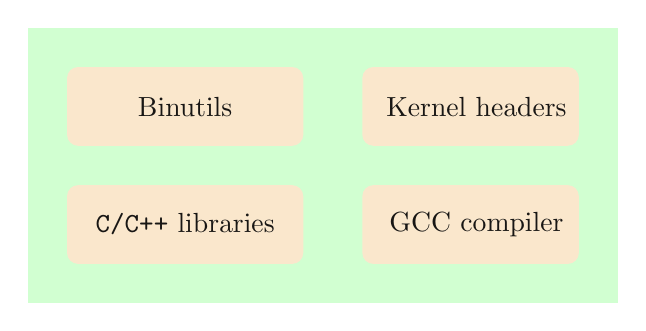
\begin{tikzpicture}[fill opacity=0.9]
		\fill[green!20] (0.25,0.25) rectangle (7.75, 3.75);

		\fill[orange!20, rounded corners] (0.75,2.25) rectangle (3.75, 3.25);
		\draw (2.25, 2.75) node {Binutils};

		\fill[orange!20, rounded corners] (4.5,2.25) rectangle (7.25, 3.25);
		\draw (5.95, 2.75) node {Kernel headers};

		\fill[orange!20, rounded corners] (0.75,0.75) rectangle (3.75, 1.75);
		\draw (2.25, 1.25) node {\texttt{C/C++} libraries};

		\fill[orange!20, rounded corners] (4.5,0.75) rectangle (7.25, 1.75);
		\draw (5.95, 1.25) node {GCC compiler};
	\end{tikzpicture}
\end{figure}

\subsubsection{A brief discussion on the ARM GNU toolchain}

A toolchain can usually be described by a quadruple taking the general format \texttt{<arch>}-\texttt{<vendor>}-\texttt{<os>}-\texttt{<libc/abi>}. \texttt{<arch>} stands for the target CPU architecture for the binaries that will be produced by the toolchain, the system manufacturer or vendor who is responsible for the hardware is \texttt{<vendor>}, \texttt{<sys>} generally stands for the operating system or takes the special value "none" for bare-metal, and the target application binary interface or \texttt{C} runtime is \texttt{<libc/abi>}. This tradition of naming toolchains exists across build automation tools, compiler projects, etc in different ways under different names such as system definitions in autoconf, or the target triple in LLVM\textquotesingle s Clang.

ARM GNU toolchain is a GNU toolchain for ARM architecture that is released and maintained by ARM and from open-source project GCC, Binutils, glibc, Newlib, and GDB. The toolchain supports \texttt{C} and \texttt{C++} languages and supports CPUs based on the 3 main flavours of processor cores namely the Cortex A, Cortex R, and Cortex M.

\begin{table}[h]
	\centering
	\begin{tabular}{ |p{7em}|p{9em}|p{12em}| }
		\hline
			\textbf{Processor Core} & \textbf{ARM Architecture} & \textbf{ARM Processor Core} \\
		\hline
			nRF51822 & ARM v6-M & ARM Cortex M0 \\
		\hline
			AM2732 & ARM v7-R & ARM Cortex R5 \\
		\hline
			AM3358 & ARM v7-A & ARM Cortex A8 \\
		\hline
			i.MX6S & ARM v7-A & ARM Cortex A9 \\
		\hline
			Kryo 240 & ARM v8-A & ARM Cortex-A73, A53 \\
		\hline
	\end{tabular}
	\caption{A few ARM application processors with their processor cores and CPU architecture}
	\label{table:arm}
\end{table}

% TODO : Add one more column on the application areas for the processor cores

\subsection{Application development using QEMU}

Another common alternative to cross compiling in this manner is by using native compilers via emulation. Emulation is some technique that allows a (host) computer system to simulate the behaviour of some other (guest) computer system. There are several software projects that allow for emulation in this manner with QEMU being by far the most commonly used emulator targetting several different hardware platforms. QEMU can also be used to create and test embedded applications before being deployed on the target hardware. Application development for embedded devices usually employs a combination of cross compiling toolchains and emulation software to create, test, and maintain the software.

\subsubsection{An example Embedded Development Environment on Linux using QEMU}

% TODO : Mention assumptions regarding the code listings (e,g, on their reliability) and state the environments in which the listings were tested in (e.g. fedora 36)

In this section let's consider a simple development environment capable of compiling and executing \texttt{C} programs for the \texttt{armv7l} ARM processor using a personal computer running linux. This setup leverages features of the Linux operating system running on the development host and the capabilities of the QEMU machine emulation system. The code listings in this section assumes a fedora workstation operating system and was tested using such a setup. The commands maybe specific to this environment, such as those for the fedora\textquotesingle s package manager utility \texttt{dnf}. However the general principles maybe used to create a similar setup on other linux distributions as well.

The Linux kernel has a feature called \texttt{binfmt\_misc} which stands for \textit{Miscellaneous Binary Format}. This feature allows for interpreter programs to be associated and invoked upon using certain binary format files. Together with the \texttt{chroot} command, \texttt{binfmt\_misc} can be leveraged to setup an environment that can use a QEMU emulator program to test and develop for a different architecture than that of the development host.

The interpreter programs registered with \texttt{binfmt\_misc} are usually user space applications such as emulators and virtual machines. For this section the intepreter program will be a QEMU user space emulator program, namely \texttt{qemu-arm}. QEMU has multiple operating modes apart from a full system emulation such as its user-mode emulation mode. In user-mode emulation, QEMU can perform system call translation and POSIX signal handling in linux which effectively allows for programs compiled for a different instruction set to be executed using QEMU. Cross compiling and cross debugging are common use cases for this user-mode emulation in QEMU. \texttt{qemu-arm} is a QEMU User space emulator program for executing programs compiled for ARM.

After an interpreter and binary file format pair are registerd, \texttt{binfmt\_misc} recognises the associated binary files by matching some bytes at the begining of a file with a magic byte sequence that had been supplied. The usage of magic bytes at the begining of files is a UNIX tradition adopted as a means of incorporating file type metadata within the file.

As with some linux features, \texttt{binfmt\_misc} must first be mounted at specific location after which it can be configured.

\begin{minted}{bash}
mount binfmt_misc -t binfmt_misc /proc/sys/fs/binfmt_misc
\end{minted}

To register the binary format and interpreter pair to setup the development environment, a string of the form \texttt{:name:type:offset:magic:mask:interpreter:flags} needs to be send (\texttt{echo}ed) to the \texttt{register} file at the path mentioned previously. Assuming that \texttt{qemu-arm} is present at the path \texttt{/usr/bin}, running the following command will register \texttt{qemu-arm}

\begin{minted}{bash}
echo ":qemu-arm:M::\x7fELF\x01\x01\x01\x00\x00\x00" "\x00\x00\x00\x00\x00\x00\x02\x00\x28\x00:" "\xff\xff\xff\xff\xff\xff\xff\x00\xff\xff" "\xff\xff\xff\xff\xff\xff\xfe\xff\xff\xff:" "/usr/bin/qemu-arm-static:F" > /proc/sys/fs/binfmt_misc/register
\end{minted}

Note that the \texttt{echo} should produce a string without whitespaces. A new file named \texttt{qemu-arm} will show up in the path \texttt{/proc/sys/fs/binfmt\_misc/} upon successful completion of the \texttt{echo} command.

Another linux feature is \texttt{chroot} which allows for changing the apparent root directory of a running process and its children. \texttt{chroot} system call interface started with UNIX and is useful for testing and developing software systems in a modified test environment.

Prior to running \texttt{chroot}, a root directory for the target environment must be prepared. A root directory is simply the top most directory in a hierarchy and can be prepared by sourcing programs and packages necessary for developing \texttt{C} programs for \texttt{armv7l}. Sourcing these programs can be a matter of approaching maintainers of the packages who may provide the appropriate binaries or building them from source using a cross compiler.

For example, versions of the fedora linux distribution provides these packages via its packages manager and the following command can source the necessary programs for that architecture.

\begin{minted}{bash}
dnf install --releasever=36 --installroot=/tmp/f36arm --forcearch=armv7hl --repo=fedora --repo=updates systemd passwd dnf fedora-release vim-minimal m4 cmake gcc-c++ tar gcc git make tmux -y
\end{minted}

The target directory \texttt{/tmp/f36arm/} will then contain a simple root directory for the required development environment for \texttt{armv7l}. After configuring the environment in this manner, simply test changing the root directory and running a simple \texttt{C} program.

\begin{minted}{bash}
chroot /tmp/f36arm /usr/bin/bash
\end{minted}

Since the \texttt{C} compiler for \texttt{armv7l} has been acquired for this environment using \texttt{dnf} command previously, \texttt{qemu-arm} will be able to run the compiler from the bash environment that is using QEMU\textquotesingle s user-mode emulation. A simple hello world program as shown in the listing below can then be compiled and then executed in this environment

\begin{minted}{c}
#include <stdio.h>

int main()
{
	puts("Hello, World!\n");
	return 0;
}
\end{minted}

Development environments such as these are easy to setup and can prove valuable for rapid prototyping. Another use case may be as part of a continuous integration and continuous delivery mechanism for embedded application development

\subsection{Targeting Embedded Devices}

Building an Embedded Linux kernel suited for a mainboard of an embedded device requires appropriate build configurations describing the kernel, its enabled feature, the device tree layout, i/o memory mapping, etc \cite{bootlin-port}. These parameters are a description of the devices on the mainboard, their interfaces to the processor, and the nature of the Embedded Linux that is to be managing the hardware platform. The collection of software and configurations required to get an operating system running on a board is referred to as a \textit{Board Support Package} (BSP).

% TODO : Add discussion on device tree layouts - possibly move the discussion to the Theory chapter, link to that discussion from here

To port Linux onto a processor on a particular board requires creating a boot loader capable of that task as well. A boot loader program is responsible for placing an operating system into memory and handing over the control of the processor. The technical details as to how the boot loader has to be configured will be based on the particulars of the hardware that it will be configured for.

The initial target machine for the project was an ECU filling the role of a communicator on the truck. The BSP source code for the board however was unavailable as well as certain critical support components for the board, such as the vendor's Yocto meta layer, memory mapping for the attached devices, source codes for boot ROM firmware or the boot loader, etc. The reverse engineering efforts to attain this information were dropped due to time constraints and ultimately a similiar board, namely the MCIMX6Q-SDB evaluation board, with the required information publicly provided by processor chip vendor NXP was chosen as the target platform. The details of the attempt at uncovering this information is layed out in \hyperref[rtc-c300]{Appendix II}.

\section{Neural Network Application Development}

The most popular ways to write neural network models are by using machine learning frameworks such as Tensorflow, MXNet, PyTorch, Caffe, etc. all of which have Python as their primary programming language. The Development process for neural network application in industry has several steps from collecting and preparing the data, choosing a network architecture, implementing that model, training and evaluating the model, tuning the hyperparameters of the model, deploying the model to perform inference on new data, and monitoring and improving the model. Several software components, network resources, compute devices, engineerig personnel, etc. has to come together for the effective deployment such an application.

\subsection{Choice of Programming Language and Machine Learning Framework}

As most neural network applications are written in frameworks like PyTorch and Tensorflow, they have thriving ecosystems that provide rich developer support. Most neural network models are trained in a rich compute environments with either dedicated machine learning computer systems or general purpose computer systems with plentiful operational capacities. Machine learning based companies and their service offerings such as cloud machine learning platforms almost invariably target these platforms and provide software tools for developers to utilize. Developers in these platforms enjoy several resources such as productivity tools that allows for continuous integration and development, performance profiling tools, etc.

% TODO : Consider examples from https://github.com/EthicalML/awesome-production-machine-learning

The programming environment for embedded devices however are not as featureful. Developer resources such as productivity tools for neural network application development and maintainance are lacking and the software stacks that are traditionally used are either too large or unsupported on the broader embedded hardware platforms.

Another aspect to consider is the programming language and software stack used to describe a neural network application. Most machine learning models at present are written in Python and frameworks like PyTorch and Tensorflow have richer interfaces for Python compared to other programming languages. This may be unfavourable to embedded devices where a Python application may take up higher memory and have longer latencies. The programming language of choice for embedded applications is \texttt{C} and \texttt{C++} which are supported by the ML frameworks but not to the same extent as their Python interfaces.

Machine learning frameworks also utilise multiple software libraries meant for specific aspects of performing machine learning calculations. For instance, a neural network model described in Python using Keras gets converted to a computational graph representation in Tensorflow. Then depending on the model, its invocation, and the compute platform its running on, Tensorflow determines the operations involved, execution order, etc. and execute the computation. At this stage Tensorflow may also use other software libraries such as XNNPACK, or Intel oneAPI Math Kernel Library to perform the calculations.

% TODO : Link to XNNPACK, oneAPI papers / resources

\subsection{Neural Network Inference on Embedded Devices}

The typical deployment of neural network models on embedded devices follows a pattern of gathering sensor data from the embedded device onto an external data lake, training a neural network model using this data on workstations or cloud platforms, then implementing the neural network model inference on the embedded device. Preferably the implementation utilise math kernel libraries that are made specifically for the embedded platform and the popular machine learning frameworks may provide an avenue to transfer models written in them to target the embedded platform.

The possibilities in making embedded platforms more involved in the neural network development process has been explored in research avenues such as TinyML\cite{tinyml}, and other efforts motivated by interests in getting the neural network applications ready for mobile devices such as Tensorflow Lite\cite{tfl} and PyTorch Mobile \cite{pytorch-mobile}

However the primary approach in these cases is with a focus on making the neural network model inference step faster on these embedded platforms.

% TODO : Gap in the market: No support for training ML models on embedded devices❓

\section{Federated Learning of Neural Networks}

A significant problem in the traditional model for neural network application development in embedded devices is the consumption of network bandwith associated with continual transmission of sensor data to the data lake. The data from different devices are then combined together to form the dataset that will be used to further train the model. However this stream of data coming from the embedded platform exposes the device to computer security risks such as an attacker gaining access to the behavioural data of the vehicle.

\begin{figure}[h]
	\centering
	\begin{tikzpicture}

		\node (ecu) at (0,0) {
\includegraphics[scale=2]{truck.png}};

		\node (cloud) at (3.5, 2) {
\includegraphics[scale=2]{db.png}};

		\node (server) at (7, 0) {
\includegraphics[scale=2]{server.png}};

		\draw[->,thick] (ecu) -- (cloud);
		\draw[->,thick] (cloud) -- (server);
		\draw[->,thick] (server) -- (ecu);

	\end{tikzpicture}
\end{figure}

One way to address this problem is to rely on alternative mechanisms to perform the continual training of the model in a decentralised manner. Federated learning is a technique of training ML models in such a distributed way, where each client device uses its own data set to train a local model. After this local training session, the new model may be send to a central server which will combine the different models to form a new global model. This may be then sent to the client devices for performing inference.

\begin{figure}[h]
	\centering
	\begin{tikzpicture}[rounded corners, opacity=0.87]

		\readlist\Trucks {1,2,3,4}
		\foreachitem \x \in \Trucks
		{
			\node (ecu \x) at ({0 + 2.5 * (\x-1)}, 0) {
\includegraphics[scale=2]{truck.png}};
		}

		\node[inner xsep=21pt] (server) at (3.5, 2) {
\includegraphics[scale=1.8]{server.png}};

		\foreachitem \x \in \Trucks
		{
			\draw[<->,thick] (ecu \x.north) -- (server);
		}

	\end{tikzpicture}
\end{figure}

Federated learning has several different approaches differing in the manner in which distributed training can take place, the algorithm to combine different locally trained models, and other strategies used in completing the development loop. In the LOBSTR \cite{lobstr} and FAMOUS \cite{famous} projects Scania has developed statistical models and neural network models for anomaly detection using a federated learning approach. The statistical models are lightweight and can easily be trained with limited computational resources.

This thesis focuses on repurposing existing hardwared (ECU) to ML edge devices that are tailored to train neural network in the most efficient possible way. We try to reverse engineer the old communicator model to build a custom Yocto project tailored for ML. As alternative test ECU we use an evaluation board that has similar specifications as the commuicator to benchmark and experiment different neural network implementations and evaluate.


% ============================================
%        Theory
% ============================================

\chapter{Theory}

The first section in this chapter lays out an overview of the training process of neural networks. The following section introduces some terminology associated with software development for embedded devices, contextualised in Embedded Linux.

\section{Neural Networks}

A neural network consists of a collection nodes called \textit{neurons} that are arranged into several layers with connecting edges that go between the layers. A connecting edge between two neurons describe an operation with the first neuron producing an output that is then consumed as input by the second neuron. The first layer and final layer are special and are called \textit{input layer} and \textit{output layer} respectively. There maybe zero or more layers that lie between them called \textit{hidden layers}.

\begin{center}
	\begin{tikzpicture}[x=2.4cm,y=1.2cm]
		\readlist\Shape{4,3,2}
		\readlist\Type{1,2,3}
		\readlist\Label{x,h^{(\prev)},y}

		\def\yshift{0.45}

		\foreachitem \nodes \in \Shape{
			\def\lay{\nodescnt}
			\pgfmathsetmacro\prev{int(\nodescnt-1)}

			\foreach \i [evaluate={
				\c=int(\i==\nodes);
				\y=\nodes/2-\i-\c*\yshift;
				\x=\lay;
				\n=\Type[\lay];
				}] in {1,...,\nodes} {

				\node[node \n] (nodes\lay-\i) at (\x,\y) {$\Label[\lay]$};

			\ifnum\lay>1
				\foreach \j in {1,...,\Shape[\prev]}{
				\draw[connect,white,line width=1.2] (nodes\prev-\j) -- (nodes\lay-\i);
				\draw[connect] (nodes\prev-\j) -- (nodes\lay-\i);
				}
			\fi
			}
			\path (nodes\lay-\nodes) --++ (0,1+\yshift) node[midway,scale=1.5] {$\vdots$};
		}
	\end{tikzpicture}
\end{center}

The connecting edges between the neurons are weighted and additionally a neuron may carry a weight of its own called \textit{bias}. The neurons may have several incoming edges, except for the neurons in the input layer, and several outgoing edges, except for the neurons in the output layer. Each neuron in the network describes a computation in at least two steps, (1) multiply input data with corresponding edge weight and take their sum along with the bias value, (2) transform the value calculated earlier using an activation function.

An activation function $\sigma$ is said to determine the activation of the neuron which can be thought of as the output that the neuron generates. There are several kinds of activation functions that are used in neural networks such as the sigmoid, ReLU, tanh, etc.

Combining these operations the neuron $y_k$ has the output

\begin{equation}
	y_k = \sigma \left( \sum_{j=0}^m w_{kj} x_j \right)
\end{equation}

Where $y_k$ is the $k^{th}$ neuron in a layer with input values $x_0$ through $x_m$ with corresponding weights $w_{k0}$ through $w_{km}$. The first input $x_0$ is usually set to $0$ and hence the corresponding weight $w_k0$ stands in for the bias $b_k$ of the neuron. The complete neural network matrix multiplication pass from input to output is called the \textit{feedforward}.

Neural networks can be constructed in a variety of ways with the choice for how many layers to use, the number of neurons in the layers, the connections between the layers, all of which can generate several different topologies. The neural network model can approximate a real world system by modelling that system as function that takes in some input and then generating an output. The neural network can approximate this function better by changing the connections between neurons, dropping and or adding neurons, varying the weights encoded in the connections, or by varying the biases within the neurons.

\subsection{Training a Neural Network}

One of the most interesting characteristics of a neural network is its capacity to form probability weighted associations between a set of inputs and their correponding outputs. The process of forming this association is called \textit{training} the neural network, the set of input patterns used for this purpose is called a \textit{training set}, and the algorithm by which the network is trained is called the \textit{learning algorithm}. After sufficient training, the network can also produce correct outputs to unseen inputs of the same kind.

% TODO : Give more mathematical motivations on how neural networks learn patterns

The bulk of the mathematical operations involved in training a neural network are simply addition and multiplication instructions of floating point values. Hence a computing platform that is executing a learning algorithm for some neural network is issuing a series of floating point addition and multiplication instructions. Modern computers have optimised hardware features that allow for parallel executions of these multiply and add instructions, all in an effort to improve the training efficiency of neural networks. Google's TPU chip (Figure \ref{fig:google-tpu})

\begin{figure}[h]
	\centering
	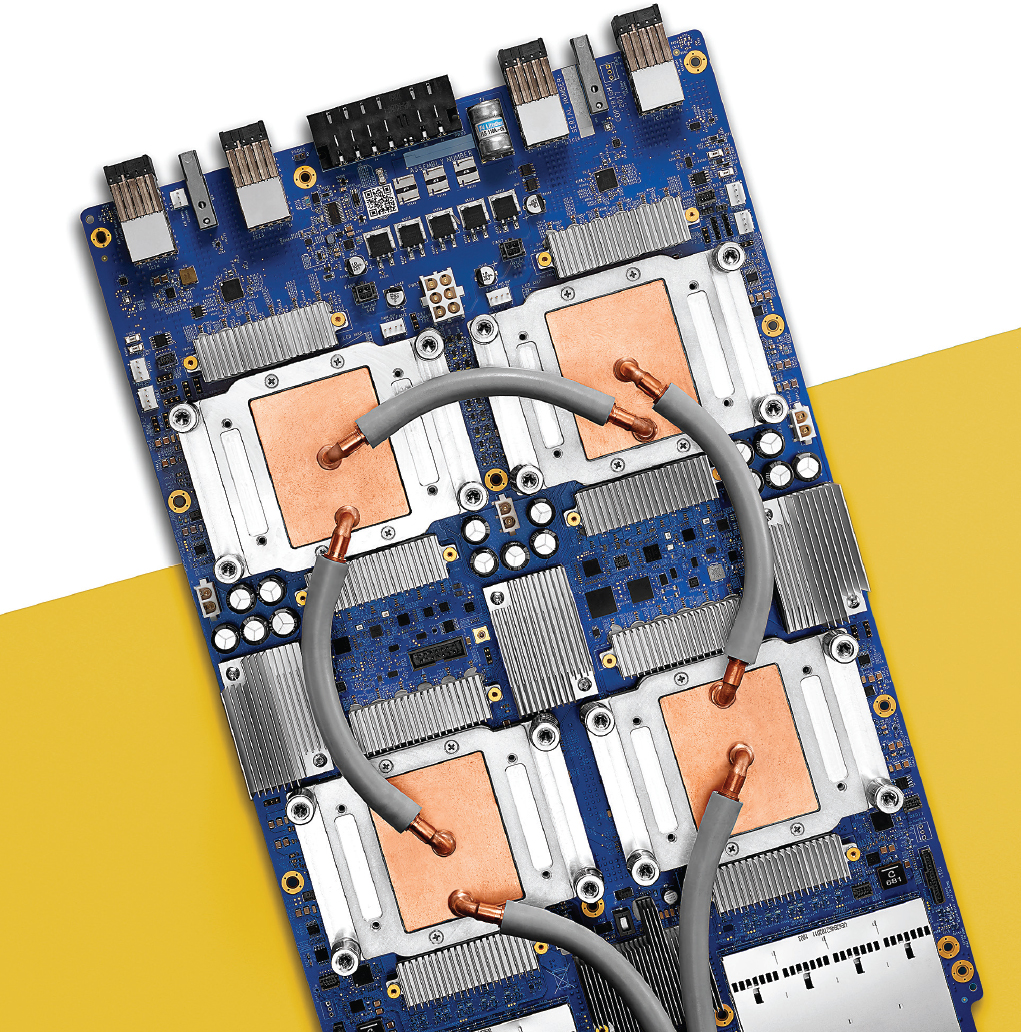
\includegraphics[scale=0.28]{google-tpu.jpeg}
	\caption{Google's TPU Chip}
	\label{fig:google-tpu}
\end{figure}

\subsection{Training vs Inference}

Once a neural network completes a training on a training set, it can then be used to look at data points that it has not seen previously. The neural network can be made to perform the feedforward calculations to produce some prediciton or output and this step is said to be a neural network \textit{inference}.

\section{Embedded Linux}

As presented in the preivous chapter, the development, deployment, and maintainance of Embedded Linux distributions and their user mode applications are usually managed using capable build systems. Configuring these systems requires understanding concepts such as boot loaders, device tree layouts, flash memory, cross compiling toolchains, board suport package, etc. with the later two having already been introduced in the preceding chapter.

Porting an Embedded Linux distribution on some embedded hardware completes successfully when the processor on the board is able to run the Linux operating system. Depending on hardware several paths may be taken by the processor to reach this stage after powering on. This process of starting the computer is called \textit{booting} and the sequence of stages the board goes through is called \textit{boot sequence}. Embedded devices are greatly varied and hence there is great variance in how boot sequence take place.

\subsection{A Simplified Boot Sequence}

After power up, the processor requires initialisation which for the kind of processors usually found in ECUs is performed by firmware placed in a special purpose memory called \textit{Boot ROM}. This code is responsible for initialising peripheral devices, hardware busses, CPU registers, etc. and after hardware initialisation locates and loads a bootloader program. Bootloader programs are responsible for continuing the boot process and may have multiple stages with one loading another. The most commonly used open source boot loader for embedded devices is U-Boot. U-Boot will normally be stored in some storage medium that will be accessible by the Boot ROM code, usually some flash memory. Flash memory is a kind of non-volatile memory that can be electrically erased and reprogrammed and is commonly used for storing data and firmware. Flash memory comes in two kinds, NOR flash and NAND flash which have different performance characteristics and usage scenarios.

\begin{figure}[h]
	\centering
	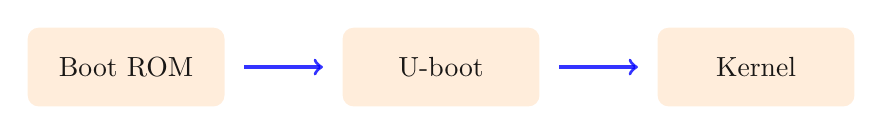
\begin{tikzpicture}[fill, rounded corners, opacity=0.7]
		\tikzset{next/.style={blue, ->, very thick, opacity=0.8}}
		\fill [orange!20] (0,0) rectangle (2.5, 1);
		\draw [opacity=0.9] (1.25, 0.5) node {Boot ROM};
		\draw [next] (2.75, 0.5) -- (3.75, 0.5);
		\fill [orange!20] (4,0) rectangle (6.5, 1);
		\draw [opacity=0.9] (5.25, 0.5) node {U-boot};
		\draw [next] (6.75, 0.5) -- (7.75, 0.5);
		\fill [orange!20] (8,0) rectangle (10.5, 1);
		\draw [opacity=0.9] (9.25, 0.5) node {Kernel};
	\end{tikzpicture}
\end{figure}

After getting control of the processor, U-Boot then has to take care of initialising the memory system, finding then loading the Linux kernel into an appropriate location in memory, generate boot parameters for the kernel, and copy other required data for the kernel. The kernel is also commonly stored on a flash memory on board. One of the configuration data that U-Boot has to pass to the kernel is the device tree, which is a data structure describing the hardware layout. Device trees were adopted in Linux and the embedded industry in general to allow mainline Linux and U-Boot to use the device tree to run on a particular board configuration, and to disuade the creation of U-Boot and Linux forks to target marginally different boards \cite{device-tree}.

Once U-Boot completes and gives up control over the processor, the kernel then starts with more configuration steps such as configuring the memory, processor, peripherals, cache, and other hardware devices. The kernel then proceeds to complete its start up by setting up Stacks, initialising the Scheduler, setting up and allocating Pages, etc. and completes the start up after having spawned the \texttt{init} process, which is the first process to that starts after booting completes.

% TODO : Include more discussion on device tree layouts (see previous TODO on device tree layouts)

\subsection{Porting Embedded Linux}

Creating the binaries for an embedded linux and managing configurations for a particular board requires a build system capable of the task. This section takes a look at one such system, namely the Yocto project.

\subsubsection{An excursion through Yocto Project's Embedded Linux build system}
\label{section:yocto-demo}

Embedded linux build systems can become fairly large and complicated software stacks depending on their supported development scenarios, number and nature of the software engineers using the tool, the build and deploy infrastructure, and the list of supported target platforms. Consider a simple development scenario targetting the popular and open source embedded target platform MCIMX6Q-SDB. The aim is to build and run an embedded linux distribution for the MCIMX6Q-SDB using a personal computer running linux. Note that several components used in this discussion may break their interface so the emphasis will be on the essential concepts of the activites involved.

\begin{figure}[h]
	\centering
	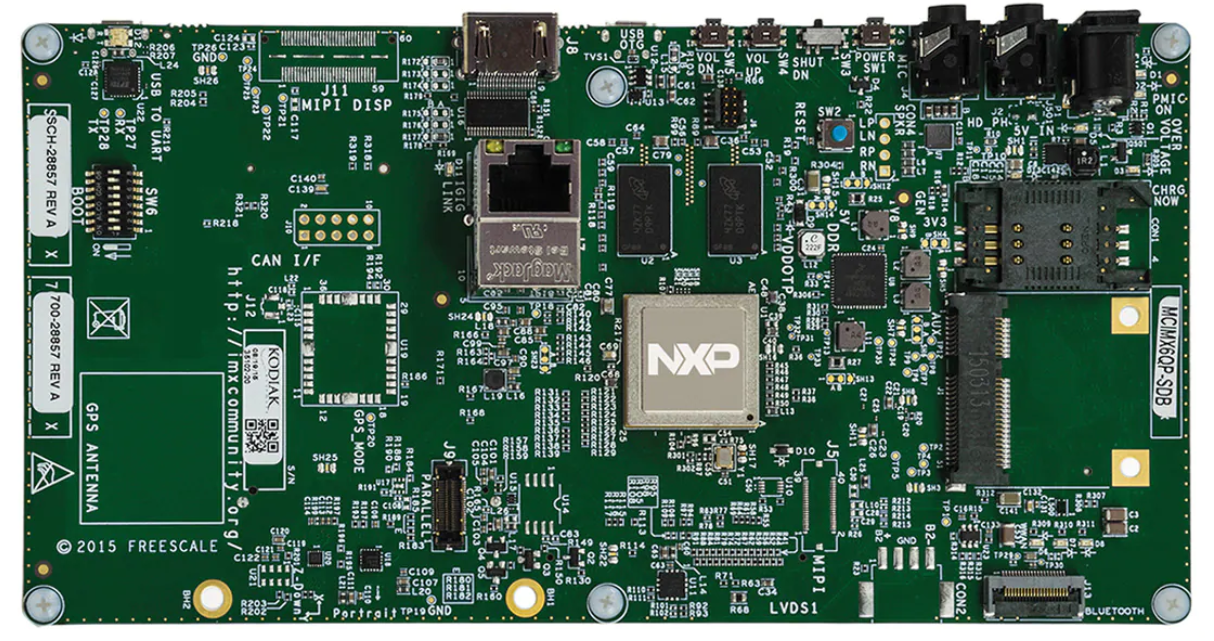
\includegraphics[scale=0.32]{MCIMX6Q-SDB-BD.png}
	\caption{MCIMX6Q-SDB-BD}
	\label{fig:mcimx6q-sdb}
\end{figure}

The Yocto Project is arranged into several components out of which the core 3 components are BitBake, OpenEmbedded-Core, and Poky. BitBake is a build engine that interprets configuration files to schedule and then perform tasks. These configuration files are called \textit{recipes} and they describe how to build a particular package such as a shared library or application program. Recipes contain information as to where to obtain the source code for a package, instructions for compiling the source code, and installing or removing that package from a distribution. OpenEmbedded-Core is a set of platform and distribution independent recipes and other metadata while Poky is a reference system containing a collection of projects and tools that can be used to bootstrap a new distribution.

The Yocto Project came out of the work associated with OpenEmbedded build automation framework and shares maintainership of the central parts of the OpenEmbedded build system with the OpenEmbedded project. OpenEmbedded-Core came out of a split of the recipe metadata held within OpenEmbedded. The big picture of the Yocto project can be fairly complex and the amount of terminology and techniques associated with using the project causes the Yocto project to have a steep learning curve. A simplified illustration of the Yocto project is presented in Figure \ref{fig:yocto-overview} below. A set of recipes (teal) sharing a common purpose are arranged into a \textit{layer} (cyan) \ref{fig:yocto-overview}. Layers can depend on other layers, with multiple layers usually being used in an embedded linux distribution.

\begin{figure}[h]
	\centering
	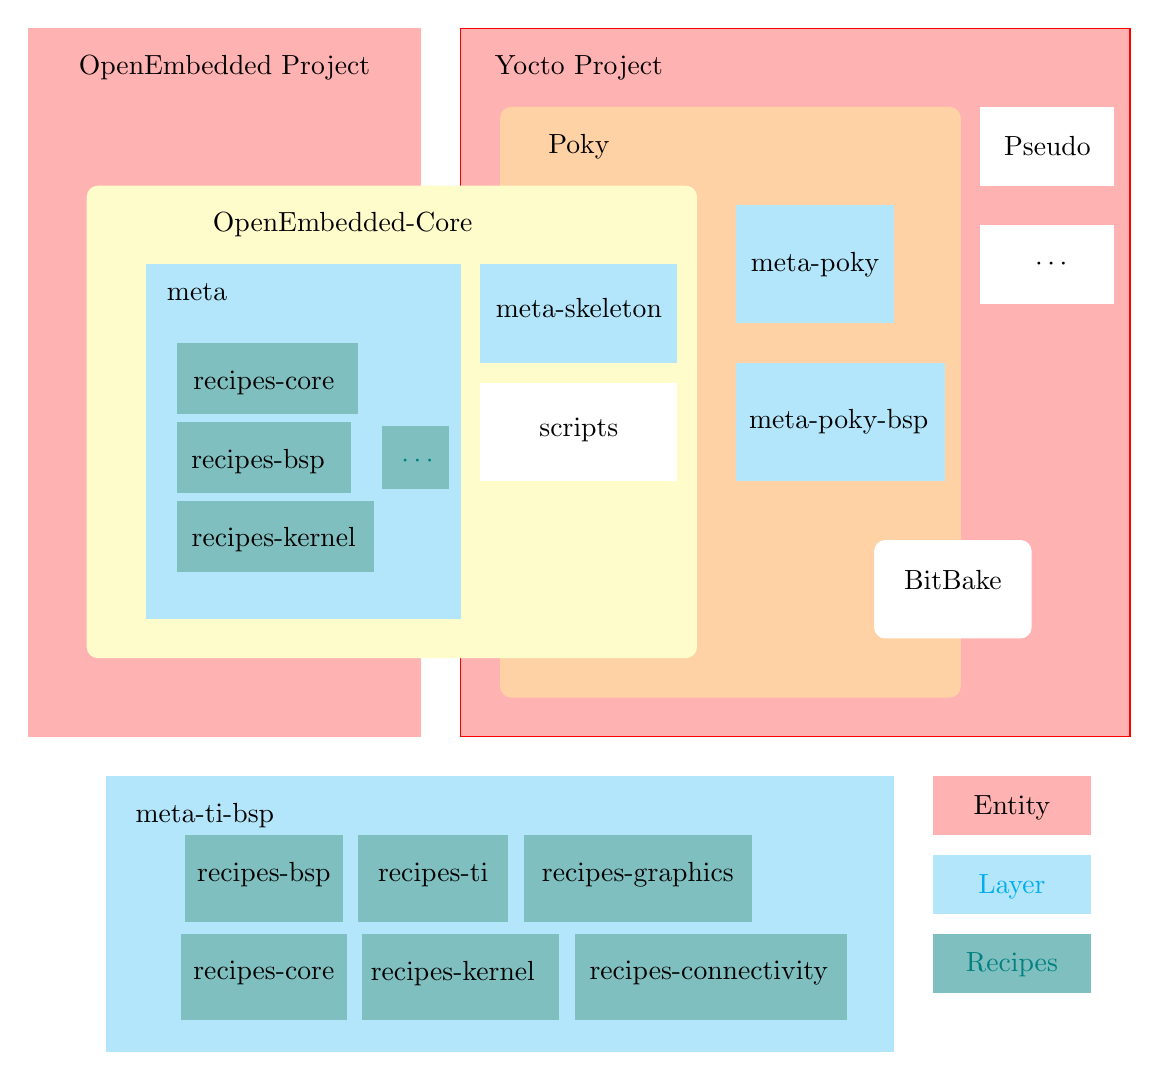
\begin{tikzpicture}
		\fill[fill=red!30] (0, 0) rectangle (5, 9);
		\draw (2.5, 8.5) node {OpenEmbedded Project};

		\draw[fill=red!30, draw=red] (5.5, 0) rectangle (14, 9);
		\draw (7, 8.5) node {Yocto Project};

		\fill[orange!35, rounded corners] (6, 0.5) rectangle (11.85, 8);
		\draw (7, 7.5) node {Poky};

		\fill[yellow!20, rounded corners] (0.75, 1) rectangle (8.5, 7);
		\draw (4, 6.5) node {OpenEmbedded-Core};

		\fill[cyan!30] (1.5, 1.5) rectangle (5.5, 6);
		\draw (2.15, 5.65) node {meta};

		\fill[teal!50] (1.9, 4.1) rectangle (4.2, 5);
		\draw (3, 4.5) node {recipes-core};

		\fill[teal!50] (1.9, 3.1) rectangle (4.1, 4);
		\draw (2.925, 3.5) node {recipes-bsp};

		\fill[teal!50] (1.9, 2.1) rectangle (4.4, 3);
		\draw (3.125, 2.5) node {recipes-kernel};

		\fill[teal!50] (4.5, 3.15) rectangle (5.35, 3.95);
		\draw (4.95, 3.5) node[text=teal] {$\cdots$};

		\fill[cyan!30] (5.75, 4.75) rectangle (8.25, 6);
		\draw (7, 5.45) node {meta-skeleton};

		\fill[white!40] (5.75, 3.25) rectangle (8.25, 4.5);
		\draw (7, 3.9) node {scripts};

		\fill[cyan!30] (9, 5.25) rectangle (11, 6.75);
		\draw (10, 6) node {meta-poky};

		\fill[cyan!30] (9, 3.25) rectangle (11.65, 4.75);
		\draw (10.3, 4) node {meta-poky-bsp};

		\fill[white!40, rounded corners] (10.75, 1.25) rectangle (12.75, 2.5);
		\draw (11.75, 2) node {BitBake};

		\fill[white!40] (12.1, 7) rectangle (13.8, 8);
		\draw (12.95, 7.5) node {Pseudo};

		\fill[white!40] (12.1, 5.5) rectangle (13.8, 6.5);
		\draw (13, 6) node {$\cdots$};

		\fill[cyan!30] (1, -4) rectangle (11, -0.5);
		\draw (2.25, -1) node {meta-ti-bsp};

		\fill[teal!50] (2, -2.35) rectangle (4, -1.25);
		\draw (3, -1.75) node {recipes-bsp};

		\fill[teal!50] (4.2, -2.35) rectangle (6.1, -1.25);
		\draw (5.15, -1.75) node {recipes-ti};

		\fill[teal!50] (6.3, -2.35) rectangle (9.2, -1.25);
		\draw (7.75, -1.75) node {recipes-graphics};

		\fill[teal!50] (1.95, -3.6) rectangle (4.05, -2.5);
		\draw (3, -3) node {recipes-core};

		\fill[teal!50] (4.25, -3.6) rectangle (6.75, -2.5);
		\draw (5.4, -3) node {recipes-kernel};

		\fill[teal!50] (6.95, -3.6) rectangle (10.4, -2.5);
		\draw (8.65, -3) node {recipes-connectivity};

		\fill[red!30] (11.5, -1.25) rectangle (13.5, -0.5);
		\draw (12.5, -0.9) node {Entity};

		\fill[cyan!30] (11.5, -2.25) rectangle (13.5, -1.5);
		\draw (12.5, -1.9) node[text=cyan] {Layer};

		\fill[teal!50] (11.5, -3.25) rectangle (13.5, -2.5);
		\draw (12.5, -2.9) node[text=teal] {Recipes};
	\end{tikzpicture}
	\caption{Overview of The Yocto Project Components}
	\label{fig:yocto-overview}
\end{figure}

The primary version control system used within the Yocto project is git. The Yocto project has even several software packages requirements for its build system layed out in its documentation (see \href{https://docs.yoctoproject.org/}{docs.yoctoproject.org}). Furthermore there are minimum version for the required packages for a corresponding version of the Yocto project (see \href{https://wiki.yoctoproject.org/wiki/Releases}{wiki.yoctoproject.org/wiki/Releases}).

The following listing presents the typical required packages however, based on the linux distribution of the development host the command will vary.

% TODO : Make the listings more specific to Fedora for e.g, create new listing type with slightly different background for the _general idea_ listing

\begin{minted}{bash}
PACKAGE_MANAGER install bc make automake gcc gcc-c++ chrpath cpio diffstat gawk git python texinfo wget zstd lz4
\end{minted}

The above list is not complete and relies on non standard package names. Consulting the documentation above will provide more accurate instructions as to the packages that are necessary to start with the Yocto project.

For this section, consider the \texttt{kirkstone} Long Term Support (LTS) release of the Yocto project. To begin clone the Poky repository from \href{https://git.yoctoproject.com}{git.yoctoproject.com}

\begin{minted}{bash}
git clone https://git.yoctoproject.org/git/poky
\end{minted}

The Poky repository contains the OpenEmbedded-Core as well as the BitBake tool that is required for the build. NXP (previously freescale) is the system maker and system vendor for the MCIMX6Q-SDB and they provide a BSP layer in Yocto via the meta-freescale repository.

\begin{minted}{bash}
git clone https://git.yoctoproject.org/git/meta-freescale
\end{minted}

Checkout the kirkstone version of all the different components by checking out the corresponding branches.

\begin{minted}{bash}
git checkout kirkstone-4.0.10
\end{minted}

Once the correct branches has been checked out, the next step is to bring the BitBake tool into the shell environment. The Poky repository contains scripts that facilitate this step. Create a directory to manage the build configuration and output files and run the setup script inside the Poky repo.

\begin{minted}{bash}
source poky/oe-init-build-env $BUILDDIR
\end{minted}

The script will setup BitBake along with some additional tools and scripts in the current shell environment and also creates a few directories in \texttt{\$BUILDDIR} along with some configuration files. The first configuration file to edit will be the \texttt{\$BUILDDIR/conf/bblayers.conf} to configure the build system for the MCIMX6Q-SDB.

\begin{minted}{bash}
	MACHINE = "imx6qdlsabresd"
\end{minted}

After \texttt{\$MACHINE} is configured correctly, BitBake can create a minimal image that can boot the MCIMX6Q-SDB building the packages for \texttt{core-image-minimal} recipe.

\begin{minted}{bash}
bitbake core-image-minimal
\end{minted}

Build images will be generated in \texttt{\$BUILDDIR/tmp/deploy/images/imx6qdlsabresd}. To boot the MCIMX6Q-SDB with the build image simply flash an SD card with the rootfs image and configure the board to boot from the SD card slot. SD-3 slot may be configured in this manner by toggling the dip switches to D1-OFF D2-ON D3,4,5,6-OFF D7-ON D8-OFF

Connecting to the board via USB-UART via a serial console terminal emulator program should then be possible after power on the MCIMX6Q-SDB.
